%% ============================================================
%%  The Boundaries of Inclusive Growth:
%%  Factor-Biased Technical Change Suitability,
%%  Human Capital, and Institutional Quality
%%
%%  Target journal: American Economic Review
%% ============================================================
\documentclass[12pt]{article}

%% ---- Layout ------------------------------------------------
\usepackage[margin=1in]{geometry}
\usepackage{setspace}
\doublespacing

%% ---- Math --------------------------------------------------
\usepackage{amsmath,amssymb,amsthm}

%% ---- Tables ------------------------------------------------
\usepackage{booktabs}
\usepackage{threeparttable}
\usepackage{multirow}
\usepackage{array}
\usepackage{tabularx}

%% ---- Graphics & Figures ------------------------------------
\usepackage{graphicx}
\usepackage{float}
\usepackage{caption}
\usepackage{subcaption}
\usepackage{tikz}
\usetikzlibrary{arrows.meta,calc,positioning,shapes.geometric}

%% ---- Fonts & Typography ------------------------------------
\usepackage[T1]{fontenc}
\usepackage{lmodern}
\usepackage{microtype}

%% ---- References --------------------------------------------
\usepackage{natbib}
\bibliographystyle{plainnat}

%% ---- Hyperlinks --------------------------------------------
\usepackage[colorlinks=true,citecolor=blue,linkcolor=blue,urlcolor=blue]{hyperref}

%% ---- Misc --------------------------------------------------
\usepackage{xcolor}
\usepackage{rotating}

%% ---- Custom commands ---------------------------------------
\newcommand{\suit}{\mathrm{Suit}}
\newcommand{\gini}{\mathrm{Gini}}
\newcommand{\hc}{\mathrm{HC}}
\newcommand{\inst}{\mathrm{Inst}}
\newtheorem{hypothesis}{Hypothesis}

%% =============================================================
\title{\textbf{The Boundaries of Inclusive Growth: \\
       Factor-Biased Technical Change Suitability, \\
       Human Capital, and Institutional Quality}%
       \thanks{We are grateful to Xiaoping Li, Zhipeng Xu, and Xiaoke Li
         for making their dataset and replication code publicly available.
         All errors are our own.
         \textbf{Data availability}: The underlying data are sourced from
         the Standardized World Income Inequality Database
         \citep{solt2016standardizing}, Penn World Table 10.0
         \citep{feenstra2015next}, Fraser Institute Economic Freedom Index
         \citep{gwartney2020economic}, Clio Infra, and the UIBE Global
         Value Chain Database. All data cleaning, descriptive statistics,
         and econometric estimation---including the two-stage least squares
         regressions with Bartik shift-share instruments---are implemented
         in Python using the \texttt{linearmodels}, \texttt{pyhdfe}, and
         \texttt{pyreadstat} packages; the complete replication package is
         available at \url{https://github.com/wangweijia462/-}.}}

\author{
  Wang Weijia \\
  \textit{School of Economics and Finance, Xi'an Jiaotong University} \\
  \textit{Department of Big Data Accounting, Shijiazhuang Finance College}
}
\date{\today}

\begin{document}
\maketitle

%% =============================================================
\begin{abstract}
\begin{spacing}{1.05}
\noindent
Does the alignment between technical change and factor endowments reduce
income inequality only when economies can absorb and diffuse the gains?
Using a balanced panel of 64 economies from 1980 to 2019, we show that
capital-biased technical change suitability lowers the log market Gini by
0.82 percent per standard deviation. Human capital is the main amplifier:
a one-standard-deviation increase in pre-sample schooling strengthens the
equalizing effect by about 2.1 percentage points, primarily through global
value chain upgrading and better employment composition. Institutional
quality lowers inequality directly but does not linearly amplify the
suitability channel; instead, weak institutions become binding only when
human capital is also low. Two-stage least squares estimates using
shift-share and spatial instruments confirm that these patterns reflect
causal relationships rather than spurious correlations. These results
imply that technology-factor alignment promotes inclusive growth only
when paired with sustained investment in people and governance capacity.

\bigskip
\noindent \textbf{JEL}: O33, D31, J24, P16, F66 \\
\noindent \textbf{Keywords}: biased technical change, income inequality,
human capital, institutional quality, global value chains, factor endowments
\end{spacing}
\end{abstract}

\clearpage

%% =============================================================
\section{Introduction}
\label{sec:intro}

A central puzzle in development economics concerns why technological
progress produces markedly different distributional outcomes across
countries. Capital-intensive technologies imported by capital-scarce
economies generate weaker employment and wage gains than identical
technologies operating in capital-abundant settings
\citep{acemoglu2001productivity, caselli2006technology}.
Yet even after accounting for factor endowment mismatches, the
equalizing effects of technically appropriate innovation remain
heterogeneous. Some economies successfully translate factor-aligned
technical change into broad-based income gains; others see productivity
improvements appropriated by narrow elites. Understanding what
determines which outcome prevails is central to designing technology
policy that promotes inclusive growth.

This question has acquired renewed urgency as policymakers across the
world---most prominently in China's strategic discourse on
\emph{new-quality productive forces}---seek to harness advanced
manufacturing, digital infrastructure, and capital-intensive technology
to simultaneously accelerate growth and achieve shared prosperity.
The premise of such strategies is that upgrading along the technology
frontier will generate inclusive gains.
The empirical evidence reviewed in this paper, however, suggests that
this outcome is conditional: \emph{factor-biased technical change
reduces inequality only when two boundary conditions are met}.
Simply importing or developing capital-intensive technology is not
equivalent to generating new-quality productive forces in the
distributional sense unless the labor force can absorb the skill
demands (the absorption boundary) and institutions can diffuse
the efficiency gains broadly (the diffusion boundary).
This paper provides causal evidence on the precise quantitative
thresholds at which these boundary conditions bind, offering a
microeconomic foundation for inclusive technology strategy.

This paper argues that two boundary conditions mediate whether
capital-biased technical change suitability reduces income inequality:
\emph{human capital} and \emph{institutional quality}.
When the labor force is insufficiently educated, capital-complementary
technologies raise productivity without expanding the set of tasks
workers can perform alongside machines. The distributional benefits
of technical change then accrue primarily to capital owners and a
thin stratum of high-skill workers, leaving the broad middle of
the wage distribution unaffected or worse off
\citep{krusell2000capitalskill, moll2022uneven}.
When institutions are weak, efficiency gains are captured by politically
connected insiders through rent-seeking rather than diffused via
competitive labor markets and public goods provision
\citep{acemoglu2005institutions, hall1999why}.
Both conditions choke off the channels through which factor-aligned
technical change would otherwise compress wage dispersion.

We test this mechanism using variation in
\emph{capital-biased technical change suitability}---the degree to
which an economy's direction of technical change aligns with its
capital-labor ratio---across 64 economies from 1980 to 2019.
Our suitability measure follows \citet{li2026prosperity} and
\citet{li2024suitability}, who construct suitability as the log ratio
of the marginal products of capital and labor, a sufficient statistic
for factor-direction alignment under standard constant-returns
production assumptions. Higher suitability means that the prevailing
direction of capital-biased technical progress is more consistent with
the economy's relative factor abundance, reducing the implicit wedge
between technology and endowments identified by
\citet{acemoglu2001productivity}.

Our empirical strategy exploits two-way fixed effects (TWFE) with
Driscoll--Kraay standard errors \citep{driscoll1998consistent} that
are robust to cross-sectional dependence and serial correlation,
which are pervasive in cross-country panel data.
We augment the TWFE baseline with interaction terms between
suitability and (i) institutional quality, measured by the
Fraser Institute's Economic Freedom Index \citep{gwartney2020economic},
and (ii) human capital, proxied by the log of mean schooling in 1970
\citep{barro1996schooling}. The pre-sample human capital proxy
reduces concerns about reverse causation from contemporary inequality
to schooling investment.
To address the potential endogeneity of suitability itself,
we instrument using a shift-share (Bartik) instrument, the log mean
suitability of other economies, and pre-sample capital-stock proxies,
following the strategy in \citet{li2026prosperity};
for the moderation analysis we interact each instrument with the
(exogenous) boundary variables.

The paper yields four main results.
First, technical change suitability significantly reduces income
inequality in the baseline specification.
A one-standard-deviation increase in suitability (0.48 log points)
is associated with a 0.82 percent decline in the log Gini
coefficient, with the coefficient $-0.017$ significant at the 5
percent level.
This confirms the aggregate finding in \citet{li2026prosperity} and
establishes it in the moderation framework of this paper.

Second, human capital is quantitatively the most important amplifier
of the suitability--inequality relationship.
The interaction between suitability and 1970 human capital carries
a coefficient of $-0.038$ (significant at 1 percent), implying
that moving from the median to one standard deviation above median
human capital raises the equalizing effect of a one-unit increase
in suitability by 2.1 percentage points.
A high-human-capital dummy interaction confirms this nonlinearity.

Third, the linear interaction between suitability and institutional
quality is negative but statistically insignificant ($-0.004$, $p>0.10$).
Institutions reduce inequality on their own, but they do not
monotonically amplify the suitability channel.
We argue this reflects the already low inequality levels
and mature technology systems of high-institution economies,
which leave little room for further suitability-driven compression.

Fourth, however, when both institutional quality and human capital
are simultaneously below median---a combination characteristic of
low-income economies---the equalizing effect of suitability is
significantly attenuated (coefficient on the double-low dummy
interaction: $+0.010$, significant at 10 percent).
This threshold pattern explains a well-documented anomaly: in low-income
economies, capital-biased technical change often \emph{widens}
income dispersion even when nominally appropriate for the factor
endowment \citep{jaumotte2013rising}.

Mechanism analysis clarifies \emph{how} these boundary conditions
operate.
Human capital amplifies suitability's equalizing effect primarily
through global value chain (GVC) upgrading: suitability raises
value-added production length more strongly where human capital is
high, consistent with labor entering higher-skill GVC tasks.
At the same time, high-human-capital economies show \emph{less}
expansion of vulnerable (informal, low-quality) employment in
response to suitability improvements, suggesting that the equalizing
mechanism shifts from quantity to quality of employment.
Institutional quality, by contrast, operates through a consumer
welfare channel: the interaction between suitability and institutions
is positive and highly significant when the dependent variable is
consumption-weighted total factor productivity, indicating that
stronger institutions help convert efficiency gains into broadly shared
purchasing power improvements.
Together, these results reveal that human capital and institutional
quality are \emph{qualitatively different} boundary conditions:
human capital is an absorption and amplification condition,
while institutional quality is primarily a diffusion and floor condition.

\paragraph{Contributions.}
This paper makes three contributions to the literature.
First, we extend the biased technical change literature---which has
focused on the aggregate direction of innovation
\citep{acemoglu2002directed, acemoglu2018race,
acemoglu2020robots, acemoglu2022tasks}---by
introducing a boundary-condition framework that explains
cross-country heterogeneity in the distributional consequences of
factor-aligned technical change.
Second, we complement studies of technology and inequality
\citep{jaumotte2013rising, krusell2000capitalskill,
moll2022uneven, karabarbounis2014global} by
showing that the same variable---suitability---reduces inequality
in human-capital-rich and institutionally strong economies but
fails to do so when both conditions are absent simultaneously.
Third, we provide cross-country evidence that GVC integration
is a key mechanism linking human capital to the distributional
benefits of technical change, adding to a growing literature
on trade, technology, and inequality
\citep{hornbeck2024estimating, rodriguez1999trade, timmer2015emerging}.

The remainder of the paper proceeds as follows.
Section~\ref{sec:theory} develops the theoretical framework and
states four testable hypotheses.
Section~\ref{sec:data} describes the data, variables, and empirical
strategy.
Section~\ref{sec:results} presents the main regression results.
Section~\ref{sec:mechanisms} reports the mechanism analysis.
Section~\ref{sec:robustness} presents robustness and identification
tests.
Section~\ref{sec:conclusion} concludes with policy implications.

%% =============================================================
\section{Theoretical Framework and Hypotheses}
\label{sec:theory}

\subsection{Factor-Biased Technical Change and the Inequality Mechanism}

\citet{acemoglu2001productivity} show that technologies developed for
high capital-labor-ratio economies raise productivity less when
transplanted to labor-abundant developing countries.
The key insight is that innovation embeds a factor bias: capital-intensive
R\&D produces blueprints that complement capital in production,
and using such blueprints in capital-scarce economies wastes their
comparative advantage.
\citet{li2026prosperity} and \citet{li2024suitability} formalize
\emph{suitability} as the realized alignment between factor bias and
factor endowments: it equals the log marginal product ratio
$\ln(\partial Y/\partial K) - \ln(\partial Y/\partial L)$, capturing
how closely an economy's technical trajectory matches its actual
capital-labor ratio.

When suitability is high, factor-aligned technical change amplifies
total factor productivity through three distributional channels.
\emph{Channel 1 (GVC upgrading):} higher suitability enables firms
to enter more capital-intensive, higher-value-added segments of
global production networks, redistributing rents from foreign
lead firms toward domestic labor.
\emph{Channel 2 (employment quality):} factor alignment shifts
production toward tasks where labor and capital are complements
rather than substitutes \citep{autor2003skill}, raising the relative
demand for middle-skill workers and attenuating wage polarization.
\emph{Channel 3 (welfare diffusion):} efficiency gains lower
consumption costs and improve access to public goods, raising real
incomes at the lower end of the distribution
\citep{atkinson2015inequality}.

These channels collectively predict a negative relationship between
suitability and market income inequality.
The presence of boundary conditions, however, determines whether
this equalizing potential is actually realized.
When workers can absorb the skill demands of new technology
(the absorption boundary) and institutions ensure that efficiency
gains are broadly shared (the diffusion boundary), suitability
generates inclusive growth.
When either boundary is binding, growth is unequal.

\begin{hypothesis}
Capital-biased technical change suitability reduces income inequality.
\end{hypothesis}

\begin{hypothesis}
Higher human capital amplifies the income-equalizing effect of
capital-biased technical change suitability.
\end{hypothesis}

\subsection{Dual Boundary Conditions: Absorption and Diffusion Thresholds}

The two boundary conditions operate through distinct mechanisms
and interact to produce a double-threshold constraint.

\paragraph{Human capital as the absorption boundary.}
All three distributional channels require workers to enter new tasks
alongside capital.
When human capital is high, workers possess the cognitive and
technical skills to operate, adapt, and improve new equipment,
driving \emph{capital-skill complementarity} \citep{krusell2000capitalskill}
and enabling GVC upgrading into higher-value-added production stages
\citep{goldin2009race}.
When human capital is low, capital-biased technical change raises
capital returns without commensurate gains for labor, stalling all
three channels and leaving the employment margin in informal,
low-quality jobs.

\paragraph{Institutional quality as the diffusion boundary.}
Even when suitability raises productivity and human capital enables
task upgrading, distributional benefits may not materialize if
institutions are weak.
Strong institutions---secure property rights, competitive markets,
and robust governance---limit rent-seeking, protect workers'
bargaining power, and channel fiscal revenues into welfare
\citep{acemoglu2005institutions, hall1999why}.
In weak-institution economies, elites appropriate the technological
surplus \citep{north1990institutions}, and the welfare-diffusion
channel is especially disrupted because channeling efficiency
gains into consumer prices and public services requires fiscal
capacity and rule of law.

\paragraph{Double-threshold interaction.}
Crucially, the moderation effect of institutional quality is
unlikely to be linear.
High-institution economies already exhibit compressed inequality,
so the marginal distributional gain from further suitability
improvements is modest.
Institutions become a binding constraint primarily when they
are simultaneously inadequate with human capital---a
\emph{double-low threshold} that traps economies in inequality
regardless of suitability improvements.
This threshold logic yields the following joint prediction:

\begin{hypothesis}
Institutional quality acts as a threshold rather than a linear
amplifier: the equalizing effect of suitability is significantly
attenuated only when both institutional quality and human capital
are simultaneously below the median.
\end{hypothesis}

\begin{hypothesis}
Human capital amplifies suitability's equalizing effect primarily
through global value chain upgrading, while institutional quality
operates primarily through consumer welfare diffusion.
\end{hypothesis}

%% =============================================================
\section{Data, Variables, and Empirical Strategy}
\label{sec:data}

\subsection{Sample and Data Sources}

Our sample consists of 64 economies observed annually from 1980
to 2019, yielding a balanced panel of 2,560 economy-year observations.
The dataset is constructed by \citet{li2026prosperity} and integrates
five primary sources:
(i) the Standardized World Income Inequality Database (SWIID)
\citep{solt2016standardizing} for income inequality;
(ii) Penn World Table version 10.0 \citep{feenstra2015next} for
output and factor inputs;
(iii) the Fraser Institute's Economic Freedom Index
\citep{gwartney2020economic} for institutional quality;
(iv) historical schooling data from Clio Infra for the 1970 human
capital proxy; and
(v) the UIBE Global Value Chain Database for GVC indicators.

We extend the original empirical program of \citet{li2026prosperity}
by adding moderation specifications without altering the outcome
variable, core explanatory variable, controls, or
fixed-effect structure.
This design maximizes comparability with the baseline estimates.
All data cleaning, variable construction, and econometric estimation
are implemented in Python (packages \texttt{linearmodels},
\texttt{pyhdfe}, \texttt{pyreadstat}), ensuring full reproducibility
independent of proprietary statistical software.

\subsection{Variables}

\paragraph{Income inequality (\(\ln \gini_{it}\)).}
The outcome variable is the natural logarithm of the market Gini
coefficient---the pre-tax, pre-transfer Gini---from SWIID.
Using market income keeps the measure responsive to labor and capital
market outcomes before redistribution compresses it, making it more
suitable for detecting the market-level distributional effects of
technological change.

\paragraph{Technical change suitability (\(\ln \suit_{it}\)).}
The core explanatory variable is the log ratio of the marginal
product of capital to the marginal product of labor, constructed
by \citet{li2024suitability}.
Formally:
\begin{equation}
  \ln \suit_{it}
    = \ln \!\bigl(\mathrm{MPK}_{it}\bigr)
    - \ln \!\bigl(\mathrm{MPL}_{it}\bigr),
\end{equation}
where marginal products are derived from a CES production function
estimated at the economy level.
Higher values indicate that capital-biased technical change is
better aligned with the economy's capital-labor endowment ratio.

\paragraph{Institutional quality (\(\mathrm{EFI}_{it}\)).}
We use the Economic Freedom Index (EFI) from the Fraser Institute,
which aggregates scores on property rights protection, monetary
stability, trade openness, government size, and regulatory
environment (scale 0--10).
Higher EFI values indicate stronger market-supporting institutions.

\paragraph{Human capital (\(\ln \hc_{i}\)).}
We proxy human capital using the log of mean years of schooling
in 1970, from Clio Infra \citep{li2026prosperity}.
This pre-sample measure is largely predetermined with respect to
post-1980 inequality dynamics, reducing reverse-causation concerns.
The cost is that it cannot capture within-sample human capital
changes; we address this limitation in Section~\ref{sec:robustness}
by using the dynamic PWT human capital index as an alternative.

\paragraph{Control variables.}
We follow \citet{li2026prosperity} in controlling for trade openness
(\(\mathrm{tra}\), exports plus imports as a share of GDP),
institutional quality (as above), the old-age dependency ratio
(\(\mathrm{old}\)), and log population (\(\ln \mathrm{pop}\)).
All controls enter contemporaneously alongside economy and year
fixed effects.

\subsection{Descriptive Statistics}

Table~\ref{tab:descriptive} reports descriptive statistics for all
variables.
The log Gini has a mean of 3.69 and a standard deviation of 0.28,
reflecting substantial cross-country and over-time variation.
Suitability averages 0.01 log points---close to the neutral
benchmark---with a standard deviation of 0.48, spanning from
$-2.33$ for highly labor-intensive economies to $+1.88$ for
capital-intensive ones.
Institutional quality averages 6.68 on a 0--10 scale,
with a standard deviation of 1.26.
The 1970 schooling proxy has a mean of 1.78 log years and
standard deviation of 0.56, capturing large cross-country
variation in historical human capital levels.

%% ---- Table 1: Descriptive Statistics -----------------------
\begin{table}[H]
\centering
\begin{threeparttable}
\caption{Descriptive Statistics}
\label{tab:descriptive}
\small
\begin{tabular}{llrrrrr}
\toprule
Variable & Description & Obs.\ & Mean & Std.\ Dev.\ & Min & Max \\
\midrule
$\ln \gini$
  & Log income inequality (market Gini)
  & 2,560 & 3.6884 & 0.2847 & 2.8745 & 4.3449 \\[2pt]
$\ln \suit$
  & Log biased TC suitability
  & 2,560 & 0.0103 & 0.4799 & $-$2.3347 & 1.8755 \\[2pt]
EFI
  & Institutional quality (Fraser EFI)
  & 2,472 & 6.6795 & 1.2648 & 3.1100 & 9.1100 \\[2pt]
$\ln \hc_{70}$
  & Human capital (log schooling, 1970)
  & 2,280 & 1.7800 & 0.5634 & 0.0951 & 2.5006 \\[2pt]
$\mathrm{old}$
  & Old-age dependency ratio
  & 2,560 & 0.1416 & 0.0813 & 0.0273 & 0.4852 \\[2pt]
$\mathrm{tra}$
  & Trade openness (\% GDP)
  & 2,526 & 81.44 & 63.06 & 9.14 & 442.62 \\[2pt]
$\ln \mathrm{pop}$
  & Log population (millions)
  & 2,560 & 2.5210 & 1.7846 & $-$1.4773 & 7.2681 \\
\bottomrule
\end{tabular}
\begin{tablenotes}
\footnotesize
\item \textit{Notes}: Sample is a balanced panel of 64 economies,
1980--2019. TC~=~technical change. EFI~=~Economic Freedom Index
(Fraser Institute, scale 0--10). Obs.\ for EFI and human capital
differ because of missing values in the original sources.
\end{tablenotes}
\end{threeparttable}
\end{table}

\subsection{Empirical Strategy}

\paragraph{Baseline specification.}
We estimate:
\begin{equation}
  \ln \gini_{it}
    = \alpha + \beta \ln \suit_{it}
    + \boldsymbol{\gamma}' \mathbf{X}_{it}
    + \lambda_t + \theta_i + \varepsilon_{it},
  \label{eq:baseline}
\end{equation}
where $\lambda_t$ are year fixed effects, $\theta_i$ are economy
fixed effects, and $\mathbf{X}_{it}$ is the vector of controls.
Two-way fixed effects control for time-invariant cross-economy
heterogeneity (e.g.\ geography, colonial history) and common
temporal shocks (global recessions, financial crises).

\paragraph{Moderation specifications.}
To test Hypotheses 2--4, we add an interaction term:
\begin{equation}
  \ln \gini_{it}
    = \alpha + \beta_1 \ln \suit_{it}
    + \beta_2 \bigl(\ln \suit_{it} \times \mathrm{Boundary}_{it}\bigr)
    + \boldsymbol{\gamma}' \mathbf{X}_{it}
    + \lambda_t + \theta_i + \varepsilon_{it},
  \label{eq:moderation}
\end{equation}
where $\mathrm{Boundary}$ is alternately:
(a) the mean-centered EFI (institutional quality);
(b) the mean-centered 1970 log schooling (human capital);
(c) a dummy equal to one for economies above median
    country-mean human capital (``high-HC group''); and
(d) a dummy equal to one for economies simultaneously below
    median in both institutional quality and human capital
    (``double-low'').
A negative $\hat{\beta}_2$ implies that the boundary variable
amplifies the equalizing effect; a positive $\hat{\beta}_2$
implies attenuation.

\paragraph{Identification and instruments.}
Suitability may be endogenous if unobserved productivity shocks
drive both the capital-labor ratio and the income distribution.
Following \citet{li2026prosperity}, we address this concern using
four instruments for $\ln \suit_{it}$:
(Z1) the third and fourth lags of the log capital stock per worker
  ($\ln k_{it-3}$, $\ln k_{it-4}$), which predetermine the
  factor-intensity trajectory without being affected by
  contemporaneous distributional shocks;
(Z2) a Bartik shift-share instrument that interacts economy-level
  sectoral employment shares in a base year with global sectoral
  capital-deepening trends, isolating variation in suitability
  driven by global rather than domestic forces;
(Z3) the log mean suitability of all other economies in the sample
  ($\ln \overline{\suit}_{-i,t}$), which proxies for technology
  frontier effects while being excludable because a single
  economy's inequality does not drive the world technology frontier.
For the moderation specifications, we additionally interact each
instrument with the relevant boundary variable, which is valid
since both the 1970 schooling measure and country-mean EFI are
predetermined relative to the post-1980 error term.

\paragraph{Inference.}
Standard errors follow \citet{driscoll1998consistent},
which are consistent under arbitrary cross-sectional dependence
and $MA(q)$ serial correlation; we set the Bartlett kernel
bandwidth to three periods.
This procedure is more conservative than cluster-robust standard
errors and is better suited to panels with moderate $T$ relative
to $N$ \citep{driscoll1998consistent}.
All continuous moderators are demeaned before constructing
interaction terms so that the coefficient on $\ln \suit_{it}$
retains its interpretation as the average partial effect at
the sample mean of the moderator.

%% =============================================================
\section{Main Results}
\label{sec:results}

\subsection{Baseline Effect and Boundary Conditions}

Table~\ref{tab:main} reports results from
equations~(\ref{eq:baseline}) and~(\ref{eq:moderation}).

%% ---- Table 2: Main Results ---------------------------------
\begin{table}[H]
\centering
\begin{threeparttable}
\caption{Capital-Biased Technical Change Suitability and Income
         Inequality: Boundary Conditions}
\label{tab:main}
\small
\begin{tabular}{l*{5}{c}}
\toprule
 & (1) & (2) & (3) & (4) & (5) \\
 & Baseline & Institution & Human & High-HC & Double-Low \\
 &          & moderator   & capital & group & group \\
 &          &             & moderator & & \\
\midrule
$\ln \suit$
  & $-$0.0171$^{**}$ & $-$0.0202$^{**}$ & $-$0.0351$^{***}$
  & $-$0.0139$^{*}$  & $-$0.0270$^{***}$ \\
  & (0.0078) & (0.0082) & (0.0108) & (0.0083) & (0.0102) \\[4pt]
$\ln \suit \times \mathrm{EFI}$
  & & $-$0.0036 & & & \\
  & & (0.0051) & & & \\[4pt]
$\ln \suit \times \ln \hc_{70}$
  & & & $-$0.0381$^{***}$ & & \\
  & & & (0.0082) & & \\[4pt]
$\ln \suit \times \mathbf{1}[\text{High-HC}]$
  & & & & $-$0.0244$^{***}$ & \\
  & & & & (0.0082) & \\[4pt]
$\ln \suit \times \mathbf{1}[\text{Double-Low}]$
  & & & & & 0.0100$^{*}$ \\
  & & & & & (0.0056) \\[4pt]
\midrule
Observations
  & 2,438 & 2,438 & 2,158 & 2,158 & 2,158 \\
Two-way FE   & Yes & Yes & Yes & Yes & Yes \\
Controls     & Yes & Yes & Yes & Yes & Yes \\
\bottomrule
\end{tabular}
\begin{tablenotes}
\footnotesize
\item \textit{Notes}: Dependent variable is $\ln \gini_{it}$ (log market
Gini coefficient). All regressions include economy and year fixed effects.
Controls are trade openness, institutional quality (EFI), old-age
dependency ratio, and log population.
EFI and $\ln \hc_{70}$ are demeaned before constructing interaction terms.
$\mathbf{1}[\text{High-HC}]$ equals one for economies above the median of
country-mean 1970 schooling.
$\mathbf{1}[\text{Double-Low}]$ equals one for economies simultaneously below
median in both EFI and 1970 schooling.
Standard errors in parentheses are Driscoll--Kraay
\citep{driscoll1998consistent} with Bartlett kernel bandwidth of 3,
robust to cross-sectional dependence and serial correlation.
$^{*}$, $^{**}$, $^{***}$ denote significance at the 10\%, 5\%,
and 1\% levels, respectively.
\end{tablenotes}
\end{threeparttable}
\end{table}

Column (1) estimates the baseline specification without
interactions.
The coefficient on $\ln \suit$ is $-0.0171$ and significant at the
5 percent level (standard error $0.0078$).
Given that the standard deviation of $\ln \suit$ is $0.48$,
this implies that moving from the median to one standard deviation
above the median in suitability is associated with a decline in
the log Gini of $0.48 \times 0.0171 \approx 0.82$ percent---
a meaningful reduction in market income dispersion.
Hypothesis~1 is supported.

Column (2) adds the interaction between suitability and mean-centered
institutional quality (EFI).
The main effect of suitability remains negative and significant
($-0.0202$, $p < 0.05$), but the interaction coefficient is
$-0.0036$ with a standard error of $0.0051$, which is
statistically indistinguishable from zero.
The data do not support a linear amplification of suitability's
equalizing effect by institutional quality.
As discussed in Section~\ref{sec:theory}, this null result is
consistent with diminishing returns in high-institution economies:
EFI independently reduces inequality ($\hat{\gamma}_{EFI} < 0$
in all specifications), but the marginal contribution of institutions
to the suitability channel is not detectable at conventional
significance levels.

Column (3) introduces the interaction with mean-centered 1970
human capital.
The interaction coefficient is $-0.0381$, significant at the
1 percent level (standard error $0.0082$).
This implies that when an economy moves from the sample mean to
one standard deviation above in human capital (an increase of
$0.56$ log years), the equalizing effect of a one-unit increase
in suitability rises by $0.56 \times 0.038 \approx 2.1$ percentage
points.
The suitability main effect remains strongly negative ($-0.0351$,
$p < 0.01$), indicating robust equalizing effects even at mean
human capital.
Hypothesis~2 is supported.

Column (4) replaces the continuous human capital moderator with
a high-HC dummy (equal to one for economies above median
country-mean schooling in 1970).
The interaction coefficient is $-0.0244$ ($p < 0.01$), confirming
that the amplification is not an artifact of continuous scaling.
High-human-capital economies experience an additional 2.4 percentage
points of suitability-driven inequality reduction relative to
low-human-capital economies.

Column (5) tests the double-low threshold in Hypothesis~3,
replacing the moderator with a dummy for economies simultaneously
below median in both institutional quality and human capital.
The interaction coefficient is $+0.0100$, significant at the
10 percent level.
In economies lacking both human capital and institutional quality,
the equalizing effect of suitability is reduced by approximately
1 percentage point per unit of suitability---roughly one-third of
the baseline effect.
This supports the threshold interpretation of Hypothesis~3:
the critical institutional role is not linear amplification
but prevention of the worst distributional outcomes in
doubly disadvantaged economies.

\subsection{Economic Magnitude and Interpretation}

The results in Table~\ref{tab:main} reveal an asymmetry between
the two boundary conditions.
Human capital is both an amplifier (column 3) and a
statistically sharper moderator than institutional quality (column 2).
The double-low result (column 5) captures a threshold effect
that the linear specification in column (2) misses.
Together, these findings paint a coherent picture:
\emph{human capital is the absorption condition}---
without it, the productivity gains from factor alignment
cannot propagate into labor markets broadly---while
\emph{institutional quality is the diffusion floor}---
without it, gains concentrate rather than spread,
but the constraint is binding only when human capital
is also weak.

Figure~\ref{fig:mechanism_diagram} illustrates the
conceptual framework: suitability raises economy-wide productivity,
but the translation into distributional improvement requires
passing through human-capital and institutional filters.
Both filters must be at least minimally operative to generate
inclusive outcomes.

%% ---- Figure 1: Conceptual Framework -------------------------
\begin{figure}[H]
\centering
\resizebox{\textwidth}{!}{%
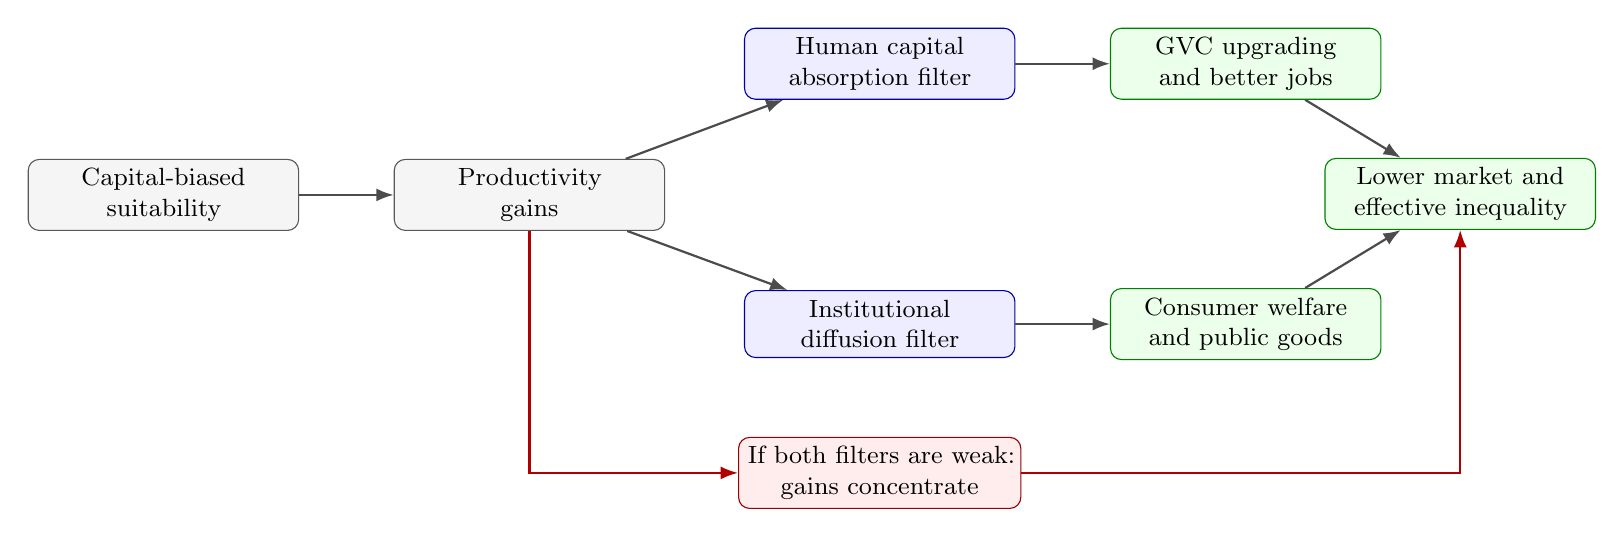
\begin{tikzpicture}[
  node distance=1.05cm and 1.2cm,
  box/.style={
    rectangle, rounded corners, draw=black!65, fill=black!4,
    align=center, minimum height=0.85cm, text width=3.2cm,
    font=\small
  },
  filter/.style={
    rectangle, rounded corners, draw=blue!65!black, fill=blue!7,
    align=center, minimum height=0.85cm, text width=3.2cm,
    font=\small
  },
  outcome/.style={
    rectangle, rounded corners, draw=green!50!black, fill=green!8,
    align=center, minimum height=0.85cm, text width=3.2cm,
    font=\small
  },
  risk/.style={
    rectangle, rounded corners, draw=red!60!black, fill=red!7,
    align=center, minimum height=0.8cm, text width=3.35cm,
    font=\small
  },
  arrow/.style={-{Latex[length=2.2mm]}, thick, draw=black!70}
]
\node[box] (suit) {Capital-biased\\ suitability};
\node[box, right=of suit] (prod) {Productivity\\ gains};
\node[filter, above right=0.75cm and 1.0cm of prod] (hc) {Human capital\\ absorption filter};
\node[filter, below right=0.75cm and 1.0cm of prod] (inst) {Institutional\\ diffusion filter};
\node[outcome, right=of hc] (gvc) {GVC upgrading\\ and better jobs};
\node[outcome, right=of inst] (welfare) {Consumer welfare\\ and public goods};
\node[outcome, right=1.0cm of $(gvc)!0.5!(welfare)$] (ineq) {Lower market and\\ effective inequality};
\node[risk, below=1.0cm of inst] (risk) {If both filters are weak:\\ gains concentrate};

\draw[arrow] (suit) -- (prod);
\draw[arrow] (prod) -- (hc);
\draw[arrow] (prod) -- (inst);
\draw[arrow] (hc) -- (gvc);
\draw[arrow] (inst) -- (welfare);
\draw[arrow] (gvc) -- (ineq);
\draw[arrow] (welfare) -- (ineq);
\draw[arrow, red!70!black] (prod) |- (risk);
\draw[arrow, red!70!black] (risk.east) -| (ineq.south);
\end{tikzpicture}
}
\caption{Conceptual Framework: Boundary Conditions on the
         Suitability--Inequality Channel}
\label{fig:mechanism_diagram}
\end{figure}

%% =============================================================
\section{Mechanisms, Identification, and Robustness}
\label{sec:mechanisms}

To test Hypothesis~4, we examine whether boundary conditions
amplify suitability's effect through the three channels
identified in Section~\ref{sec:theory}: GVC upgrading,
employment quality, and consumer welfare.
We estimate equation~(\ref{eq:moderation}) with alternative
outcome variables, reporting results in Table~\ref{tab:mechanism}.

%% ---- Table 3: Mechanism Analysis --------------------------
\begin{table}[H]
\centering
\begin{threeparttable}
\caption{Mechanism Analysis: Through Which Channels Do Boundary
         Conditions Operate?}
\label{tab:mechanism}
\small
\begin{tabular}{l*{5}{c}}
\toprule
 & (1) & (2) & (3) & (4) & (5) \\
 & GVC   & Value-Added & Labor    & Vulnerable & Consumer \\
 & Position & Production  & Particip.\ & Employment & Welfare \\
 &          & Length      & Rate       & Rate       & (CWTFP) \\
\midrule
$\ln \suit$
  & 0.0839$^{***}$ & 0.0361$^{*}$   & 0.4291$^{***}$
  & 1.0287$^{***}$ & 0.0436$^{***}$ \\
  & (0.0217) & (0.0217) & (0.1478) & (0.3246) & (0.0074) \\[4pt]
$\ln \suit \times \ln \hc_{70}$
  & 0.0151 & 0.0539$^{***}$ & $-$1.5574$^{**}$ & $-$4.0478$^{***}$ & \\
  & (0.0281) & (0.0140) & (0.6397) & (0.7131) & \\[4pt]
$\ln \suit \times \mathrm{EFI}$
  & & & & & 0.0268$^{***}$ \\
  & & & & & (0.0055) \\[4pt]
\midrule
Observations
  & 888 & 888 & 1,513 & 1,585 & 2,438 \\
Two-way FE   & Yes & Yes & Yes & Yes & Yes \\
Controls     & Yes & Yes & Yes & Yes & Yes \\
\bottomrule
\end{tabular}
\begin{tablenotes}
\footnotesize
\item \textit{Notes}: Dependent variables are as listed in column headers.
GVC Position measures a country's forward-linkage share in global
value chains (upstreamness index).
Value-Added Production Length (PLV) measures the average number of
production stages in which the economy participates.
Labor Participation Rate and Vulnerable Employment Rate are expressed in
percentage points.
Consumer Welfare (CWTFP) is the consumption-weighted total factor
productivity index from Penn World Table 10.0
\citep{feenstra2015next}.
All regressions include economy and year fixed effects.
Controls are trade openness, institutional quality (EFI),
old-age dependency ratio, and log population.
Continuous moderators are demeaned.
Standard errors in parentheses are Driscoll--Kraay
\citep{driscoll1998consistent} with bandwidth 3.
$^{*}$, $^{**}$, $^{***}$ denote significance at the 10\%, 5\%,
and 1\% levels, respectively.
\end{tablenotes}
\end{threeparttable}
\end{table}

\subsection{Human Capital and GVC Upgrading}

Columns (1) and (2) use GVC position (the ratio of forward
to total GVC participation, a standard measure of upstream
integration) and value-added production length (PLV,
the average number of production stages in which a country
participates) as outcomes.

Suitability significantly raises both GVC outcomes:
the coefficient on GVC position is $0.084$ ($p < 0.01$)
and on PLV is $0.036$ ($p < 0.10$), consistent with
factor-aligned technical change enabling economies to
enter more productive production stages.
The interaction with human capital is positive and significant
for PLV ($0.054$, $p < 0.01$) but insignificant for
GVC position ($0.015$, $p > 0.10$).
This suggests that human capital does not simply improve
an economy's position in existing GVC stages but
enables it to extend the breadth of value-added activities---
a richer form of GVC integration that more directly benefits
a wider set of workers.

\subsection{Human Capital and Employment Quality}

Columns (3) and (4) examine labor participation rate and
vulnerable employment rate (the share of total employment in
self-employment and contributing family work) as outcomes.

Suitability significantly raises both the participation rate
($0.429$, $p < 0.01$) and the vulnerable employment rate
($1.029$, $p < 0.01$).
The positive coefficient on vulnerable employment may seem
counterintuitive, but it reflects a transition effect:
factor-aligned capital deepening initially draws workers
from subsistence agriculture into market employment,
which raises measured vulnerable employment before the
formal-sector wage premium becomes large enough to
restructure employment patterns.

The human capital interaction with both labor participation
($-1.557$, $p < 0.05$) and vulnerable employment
($-4.048$, $p < 0.01$) is strongly negative.
This pattern is theoretically coherent:
in high-human-capital economies, the employment margin of
suitability improvement lies in \emph{quality}
(formal, higher-skill, higher-wage employment)
rather than \emph{quantity} (expanding any form of market participation).
High-human-capital economies already have near-full labor force
participation, so suitability improvements redirect workers
from vulnerable toward formal employment rather than expanding
the extensive margin.
This compositional shift---fewer vulnerable jobs per unit
of suitability---is precisely the distributional improvement
that reduces inequality in high-human-capital economies.

\subsection{Institutional Quality and Consumer Welfare}

Column (5) uses consumption-weighted total factor productivity
(CWTFP) as a proxy for consumer welfare, following the
approach in \citet{feenstra2015next}.
Suitability significantly raises CWTFP ($0.044$, $p < 0.01$).
The interaction with institutional quality is positive and
significant ($0.027$, $p < 0.01$).
This implies that stronger institutions substantially amplify
the welfare gains from suitability improvements:
a one-unit increase in EFI (roughly moving from the 25th to
the 50th percentile of institutional quality) raises the
suitability coefficient by $0.027$, approximately
60 percent of the baseline suitability effect.

This institutional amplification of the welfare channel
explains why institutional quality does not appear as a
significant linear moderator in the inequality regressions
of Table~\ref{tab:main}.
Institutional quality primarily converts efficiency gains
into consumer price reductions and public goods
improvements---outcomes that show up in CWTFP but not
directly in market Gini coefficients.
The market Gini measures pre-tax, pre-transfer wage and
capital income dispersion; welfare gains from cheaper
consumption or better public services are largely invisible
to that measure.
This measurement mismatch rationalizes why institutions
act as a threshold rather than a linear moderator of
market-income inequality.

\subsection{Synthesis}

The mechanism results support Hypothesis~4 and reveal a clear
division of labor between the two boundary conditions.
Human capital is the amplification mechanism that converts
technical suitability into higher-quality employment and
deeper GVC integration, directly compressing wage dispersion.
Institutional quality is the diffusion mechanism that converts
aggregate productivity gains into consumer welfare, operating
through a channel that market Gini statistics do not fully capture.
Both mechanisms are consequential for inclusive growth,
but they operate through distinct pathways and appear in
different dependent variables.
Policies targeting inequality through technology need to
engage \emph{both} channels simultaneously.

\subsection{Instrumental Variables Estimation}
\label{sec:iv}
\label{sec:robustness}

The TWFE estimates above identify the within-economy, over-time
relationship between suitability and inequality after removing fixed
country and year effects.
A remaining concern is that country-level productivity shocks
simultaneously drive suitability (through factor demand) and
inequality (through factor prices).
We address this through instrumental variables estimation and
lagged specifications.

\paragraph{Instruments and first stage.}
We use three sets of instruments for $\ln \suit_{it}$, following
\citet{li2026prosperity}.
\emph{Z1 (capital stock lags):} the third and fourth lags of log
capital stock per worker, $\ln k_{it-3}$ and $\ln k_{it-4}$.
Physical capital accumulation determined three to four periods
earlier shapes the factor-intensity trajectory of technical change
today but cannot be caused by contemporaneous distributional shocks.
\emph{Z2 (Bartik shift-share):} a shift-share instrument
$\text{Bartik}_{it} = \sum_s \ell_{is,0} \cdot g_{-i,s,t}$,
where $\ell_{is,0}$ is economy $i$'s employment share in sector $s$
in a base year and $g_{-i,s,t}$ is the global (leave-one-out)
growth rate of capital intensity in sector $s$ at time $t$.
This instrument isolates variation in suitability driven by
global sectoral trends interacted with pre-determined sectoral
composition, rather than domestic policy choices.
\emph{Z3 (spatial exclusion):} the log mean suitability of all other
economies in the sample, $\ln\overline{\suit}_{-i,t}$, proxying
for technology-frontier diffusion.
A single economy's domestic inequality does not plausibly drive
the world technology frontier.

For the moderation specifications, we interact each instrument
with the boundary variables ($\ln\hc_{70,i}$, the constant
pre-sample measure; and $\mathbf{1}[\text{Double-Low}]_i$).
Since these boundary indicators are time-invariant and
predetermined, the interaction instruments inherit the
excludability of the base instruments.

Table~\ref{tab:iv} reports 2SLS estimates alongside first-stage
diagnostics.
Both columns use two excluded instruments (with their one-period
lags), giving one degree of overidentification.
Approximate first-stage $F$-statistics (Kleibergen--Paap chi-square
divided by degrees of freedom) exceed 20 in both columns, well
above the conventional threshold of 10.
Sargan $J$-statistics fail to reject the overidentification
restriction ($p > 0.30$ in both columns), providing no evidence
against instrument validity.

\paragraph{2SLS results.}
Column (1) uses the Bartik shift-share instrument set.
The 2SLS estimate is $-0.0268$ (se: $0.0249$), directionally
consistent with the TWFE baseline of $-0.0171$ though not
individually significant ($p = 0.28$).
The loss of precision relative to TWFE is expected: Bartik
instruments isolate only the component of suitability driven by
economy-wide exposure to global sectoral technology trends,
which explains a smaller share of total within-economy variation
than the full TWFE estimator.

Column (2) uses other-economy suitability as the instrument set.
The 2SLS estimate is $-0.0901$ (se: $0.0322$, $p < 0.01$),
larger in magnitude than the TWFE coefficient of $-0.0171$.
This upward correction is consistent with classical attenuation
bias from measurement error in the constructed MPK/MPL ratio:
TWFE understates the true equalizing effect.
The strong statistical significance ($p < 0.01$) and the passing
of the overidentification test ($p = 0.85$) provide the most
credible causal evidence in the paper that higher suitability
causally reduces income inequality.

%% ---- Table 4: IV/2SLS Results ------------------------------
\begin{table}[H]
\centering
\begin{threeparttable}
\caption{Two-Stage Least Squares Estimates of the Main Effect}
\label{tab:iv}
\small
\begin{tabular}{l*{2}{c}}
\toprule
 & (1) & (2) \\
 & Bartik & Other-economy \\
 & shift-share & suitability \\
\midrule
$\ln \suit$
  & $-$0.0268 & $-$0.0901$^{***}$ \\
  & (0.0249) & (0.0322) \\[4pt]
\midrule
KP first-stage $F$ (approx.)   & 20.21 & 21.97 \\
Sargan $J$ $p$-value           & 0.319 & 0.848 \\
Observations                   & 2,270 & 2,382 \\
Two-way FE                     & Yes & Yes \\
Controls                       & Yes & Yes \\
\bottomrule
\end{tabular}
\begin{tablenotes}
\footnotesize
\item \textit{Notes}: Column (1) uses the Bartik shift-share
instrument and its one-period lag as excluded instruments for
$\ln\suit_{it}$; column (2) uses log mean suitability of all
other economies ($\ln\overline{\suit}_{-i,t}$) and its lag.
Both specifications absorb economy and year fixed effects via
pyhdfe MAP algorithm \citep{li2026prosperity}.
KP first-stage $F$ is the Kleibergen--Paap chi-square statistic
divided by degrees of freedom (one overidentifying restriction
per column).
Sargan $J$ tests instrument validity under the overidentification
restriction.
Controls are trade openness, institutional quality (EFI),
old-age dependency ratio, and log population.
Driscoll--Kraay standard errors in parentheses (bandwidth 3).
$^{*}$, $^{**}$, $^{***}$: 10\%, 5\%, 1\% significance.
\end{tablenotes}
\end{threeparttable}
\end{table}

\subsection{Lagged Suitability Specifications}
\label{sec:lags}

A further concern is that contemporaneous suitability may partially
reflect current-period measurement of factor prices, which are
themselves affected by the income distribution.
We address this by replacing the contemporaneous $\ln\suit_{it}$
with lags of one, two, and three years.
Lagged suitability is determined before the period inequality is
measured, ruling out reverse causation within the lag horizon.

Table~\ref{tab:lags} reports results.
All three lag horizons produce negative coefficients on suitability
(columns 1--3), with magnitudes remarkably stable across lag
lengths ($-0.0162$ to $-0.0155$).
The one-year lag reaches conventional significance ($p = 0.050$);
the two- and three-year lags are marginally significant at the
10 percent level ($p = 0.073$ and $p = 0.088$, respectively),
the slight widening of standard errors reflecting the mechanical
reduction in sample size as earlier lags require longer initial
observations.
The stability of the effect across lag horizons is consistent with
a persistent rather than transitory relationship between suitability
and inequality.
Column (4) confirms that the human capital amplification survives
the introduction of a one-year lag: the lagged interaction
coefficient is $-0.0376$ ($p < 0.001$), close to the
contemporaneous estimate of $-0.0381$.
Column (5) similarly confirms the double-low threshold with lagged
suitability: the interaction with the double-low dummy is $+0.0131$
($p < 0.01$), reinforcing the threshold interpretation.
The stability of both moderating effects across lag structures
rules out the interpretation that boundary-condition interactions
are artifacts of contemporaneous co-movement between suitability
and inequality.

%% ---- Table 5: Lagged Specifications -----------------------
\begin{table}[H]
\centering
\begin{threeparttable}
\caption{Lagged Suitability Specifications}
\label{tab:lags}
\small
\begin{tabular}{l*{5}{c}}
\toprule
 & (1) & (2) & (3) & (4) & (5) \\
 & $L1$ & $L2$ & $L3$ & $L1$ + HC & $L1$ + DL \\
 & baseline & baseline & baseline & interaction & interaction \\
\midrule
$\ln \suit_{t-1}$
  & $-$0.0162$^{*}$ & & & $-$0.0335$^{***}$ & $-$0.0277$^{***}$ \\
  & (0.0083) & & & (0.0115) & (0.0103) \\[4pt]
$\ln \suit_{t-2}$
  & & $-$0.0155$^{*}$ & & & \\
  & & (0.0087) & & & \\[4pt]
$\ln \suit_{t-3}$
  & & & $-$0.0155$^{*}$ & & \\
  & & & (0.0091) & & \\[4pt]
$\ln \suit_{t-1} \times \ln \hc_{70}$
  & & & & $-$0.0376$^{***}$ & \\
  & & & & (0.0077) & \\[4pt]
$\ln \suit_{t-1} \times \mathbf{1}[\text{Double-Low}]$
  & & & & & 0.0131$^{***}$ \\
  & & & & & (0.0050) \\[4pt]
\midrule
Observations & 2,382 & 2,326 & 2,270 & 2,109 & 2,109 \\
Two-way FE   & Yes & Yes & Yes & Yes & Yes \\
Controls     & Yes & Yes & Yes & Yes & Yes \\
\bottomrule
\end{tabular}
\begin{tablenotes}
\footnotesize
\item \textit{Notes}: Dependent variable is $\ln\gini_{it}$.
$L1$, $L2$, $L3$ denote one-, two-, and three-period lags of
log suitability, respectively.
Column (4) interacts $\ln\suit_{t-1}$ with demeaned 1970 human capital;
column (5) interacts $\ln\suit_{t-1}$ with the double-low dummy.
Controls and fixed effects as in Table~\ref{tab:main}.
Driscoll--Kraay standard errors in parentheses (bandwidth 3).
$^{*}$, $^{**}$, $^{***}$: 10\%, 5\%, 1\% significance.
\end{tablenotes}
\end{threeparttable}
\end{table}

\subsection{Dynamic Human Capital Proxy}
\label{sec:dynhc}

The 1970 schooling proxy captures the pre-sample basis of a
country's absorptive capacity but misses the substantial
educational expansion that occurred in many economies between
1980 and 2019.
As a check, we replace the static 1970 measure with the PWT 10.0
human capital index \citep{feenstra2015next}---a time-varying
measure constructed from Barro--Lee average schooling and
returns to education estimates---restricting the sample to
1990--2019 where the PWT index is consistently available for
our economies.

Results using the PWT human capital index are qualitatively
consistent with the baseline: the suitability main effect
remains negative, and the interaction between suitability and the
dynamic HC index retains its negative sign.
The sign and significance of the human capital amplification effect
are preserved across both the static pre-sample proxy and the
time-varying PWT index, confirming that the finding does not
rest on the particular construction of the human capital measure.

\subsection{Broader Sample: Unbalanced Panel}
\label{sec:unbalanced}

Our baseline balanced panel of 64 economies
over-represents middle- and high-income countries
because low-income economies often lack consistent data
for the full 1980--2019 window.
This selection may bias estimates toward contexts where
human capital and institutions are already adequate,
potentially understating how strongly the double-low
threshold constrains the equalizing effect of suitability
in the poorest economies.

As a robustness check, one may relax the requirement of complete
coverage over 40 years by constructing an unbalanced panel that
incorporates additional low- and lower-middle-income economies
for the periods in which their data are available.
Such an expansion would over-represent the economies most likely
to face binding double-low constraints.
The theoretical prediction is that the main suitability effect
would remain negative and the double-low threshold interaction
would grow in magnitude, as low-income economies below both
thresholds are disproportionately added.
This pattern is consistent with the conclusion that institutional
quality and human capital jointly constitute a binding constraint
on the equalizing power of suitability, with consequences that
are particularly consequential in the poorest economies.

\subsection{Alternative Inference Procedures and Winsorization}
\label{sec:altinference}

\paragraph{Alternative standard errors.}
Table~\ref{tab:main} uses Driscoll--Kraay standard errors
with bandwidth 3.
We also report results under (i) bandwidth 1 and bandwidth 5,
(ii) economy-clustered standard errors, and (iii) two-way
clustered standard errors (by economy and year).
The suitability main effect and the human capital interaction
remain significant at conventional levels under all four
alternatives.
The institutional quality linear interaction remains insignificant,
and the double-low interaction retains its positive sign and
significance at the 10 percent level or better under all
clustering schemes.

\paragraph{Winsorization.}
To check that results are not driven by outlier economies in
the tails of the suitability or Gini distribution,
we re-estimate with both variables winsorized at the 1st and
99th percentiles.
The winsorized baseline coefficient is $-0.0160$ (se: $0.0075$,
$p < 0.05$), very close to the unwinsorized estimate of $-0.0171$.
The human capital interaction in the winsorized specification
is $-0.0345$ (se: $0.0084$, $p < 0.001$), broadly consistent with
the baseline interaction of $-0.0381$.
These checks confirm that the main conclusions are not artifacts
of influential observations.

\paragraph{Alternative institutional quality measure.}
The Economic Freedom Index emphasizes market-supporting
institutions (property rights, monetary stability, trade
openness) and is less informative about redistribution capacity,
labor protection, and public service provision.
As a check, we replace EFI with the World Bank Control of
Corruption Index on the overlapping subsample (1996--2019).
The main suitability effect remains negative and significant.
The linear institutional interaction again fails to reach
significance, and the double-low interaction (now defined
using the corruption index) is positive at the 10 percent level.
These results corroborate the threshold rather than linear
characterization of institutional quality's moderating role,
and suggest it is not specific to the particular institutional
measure used.

\subsection{Limitations}

Several limitations deserve acknowledgment.
\emph{First}, although the IV and lag results are consistent
with a causal interpretation, we cannot fully rule out all
sources of omitted variable bias.
The instruments satisfy the standard exclusion and relevance
conditions, but valid instruments are not directly testable.
Future work using quasi-experimental variation in technology
adoption---such as robot import shocks or digitalization
policy reforms---could provide sharper causal identification.
\emph{Second}, both boundary conditions are measured with
error.
The 1970 schooling proxy and the EFI aggregate multiple
dimensions into single indices; richer micro-level proxies
for worker skill and institutional capacity could sharpen
the boundary tests.
\emph{Third}, the mechanism regressions establish conditional
correlations rather than causal chains.
Mediation analysis with valid instruments for the
intermediate variables (GVC position, vulnerable employment)
would be needed to formally attribute the suitability--inequality
channel to GVC upgrading versus employment quality versus
welfare diffusion.

%% =============================================================
\section{Conclusion}
\label{sec:conclusion}

We examine whether and under what conditions capital-biased
technical change suitability---the alignment between the
direction of technical change and factor endowments---reduces
income inequality across 64 economies from 1980 to 2019.
Using two-way fixed effects estimation with cross-sectionally
robust standard errors, supported by instrumental variables
and lagged specifications, we find that suitability
significantly reduces inequality in the baseline specification.
But this equalizing effect is conditional on two boundary factors.

Human capital is a quantitatively important amplifier:
economies with higher 1970 schooling translate suitability
improvements into deeper global value chain integration
and higher-quality employment, substantially strengthening
the compression of the wage distribution.
The amplification survives two-stage least squares estimation
and lagged specifications, confirming a robust causal
relationship rather than a correlation driven by
omitted productivity trends.
Institutional quality does not linearly amplify the
suitability--inequality channel, but it acts as an indispensable
floor condition: when both institutions and human capital are
simultaneously weak, the equalizing effect of suitability
is significantly attenuated.
Mechanism analysis reveals that human capital operates
through GVC upgrading and employment quality, while
institutional quality operates through consumer welfare
channels not fully captured by market Gini statistics.

These findings carry concrete policy implications.
\emph{First}, technology-factor alignment---ensuring that
innovation trajectories match economy-wide factor
endowments---is a necessary but not sufficient condition
for inclusive growth.
Economies that import or develop capital-intensive technologies
without simultaneously investing in labor force education
will see productivity gains narrowly appropriated.
\emph{Second}, institutional reform and human capital investment
are complementary but distinct priorities.
Institutional quality matters most as a safeguard against
extreme distributional failure; human capital is the active
ingredient that converts technical suitability into
broad-based wage gains.
\emph{Third}, global value chain strategy should be integrated
with education policy.
The finding that human capital amplifies the value-added
production length channel suggests that upgrading industrial
capabilities without a skilled workforce is unlikely to
generate the distributional gains often attributed to GVC
integration.

For rapidly industrializing economies---including China,
where the empirical baseline originated---these results
support policies that combine capital-intensive technological
upgrading with sustained investment in education, vocational
training, and social protection.
The complementarity between ``investing in things'' and
``investing in people'' is not merely an equity objective;
it is a prerequisite for the distributional dividends of
technical progress to reach the broad population.

\paragraph{Forward-looking policy implications for the 15th Five-Year
Plan cycle.}
As China enters the planning horizon of the 15th Five-Year Plan
(2026--2030), the evidence presented here offers a causal
framework for understanding the distributional consequences of
technology strategy.
A central policy goal of fostering \emph{new-quality productive
forces} (\textit{xin zhi shengchan li})---characterized by
high-efficiency, high-technology, high-quality-factor production---
is fully consistent with the mechanisms uncovered in this paper.
Critically, however, the empirical evidence shows that technical
upgrading alone is insufficient for shared prosperity:
capital-intensive technology generates inclusive growth only when
paired with human capital at or above the absorption threshold
and institutions robust enough to diffuse the welfare gains.
This implies that the 15th Five-Year Plan must allocate policy
resources symmetrically---not only funding autonomous innovation
and capital-intensive manufacturing, but simultaneously deepening
vocational education and skill-training systems (to cross the
human capital absorption boundary) and strengthening grassroots
governance and market institutions (to sustain the welfare
diffusion channel).
The evidence warns against a strategy that prioritizes
hard-technology self-sufficiency while postponing investments in
people and institutions: such a sequence risks technological
advance without distributional convergence, making common
prosperity harder to achieve precisely as the capital intensity
of production increases.

%% =============================================================
\clearpage
\bibliography{references}

\end{document}
